\documentclass[../../main.tex]{subfiles}

\begin{document}

\chapter{Quantum many-body framework}

This chapter is dedicated to introducing the necessary tools needed to perform realistic material calculations using DMFT or D$\Gamma$A. We start with the most central objects - the Green's functions - and subsequently assemble a complete framework which enables us to calculate a number of physical properties, e.g. the susceptibility, optical conductivity, superconductivity, pseudogaps and more, that stem from the correlated interplay between electrons or holes. 

\section{One-particle Green's functions}

Green's functions are fundamental tools in many-body physics, used to study the properties and behavior of interacting quantum systems. These mathematical objects encode information about the propagation of particles or excitations within a system and serve as the cornerstone for analyzing both equilibrium and nonequilibrium states. In the many-body regime, Green's functions extend beyond single-particle descriptions to include complex interactions among multiple particles. They provide insights into phenomena such as quasiparticle lifetimes, collective excitations and response functions. Specifically, one- and two-particle Green's functions describe the propagation of a single particle and the correlated motion of particle pairs, respectively. Alongside of the mathematical description of Green's function-based expressions, we also provide a pictorial description of the equations using Feynman diagrams. These Feynman diagrams allow us to easily describe interaction processes visually. Lines and vertices within the diagrams indicate particle propagators and interaction vertices, respectively. External legs will be coloured gray while inner legs and interaction lines will be coloured black.

In condensed matter physics, we are only interested in finite-temperature effects. Hence it is practical to use the so-called Matsubara formalism\cite{T. Matsubara. “A new approach to quantum-statistical mechanics”} in imaginary time by performing a Wick rotation $t\to -i\tau$\cite{G. C. Wick. “Properties of Bethe-Salpeter Wave Functions”}.

Furthermore, most many-body quantities described in the following are $n$-point (correlation) functions\footnote{Here, $n$ denotes the number of \say{external legs} of the corresponding Feynman diagram.}. These functions typically include a subset of the following parameters for each external leg: (Matsubara) frequency ($\nu$), spin index ($\sigma$), orbital index ($o$), lattice position ($\vv{R}$), momentum ($\vv{k}$) or imaginary time ($\tau$). This introduces a huge amount of parameters appended to a variable and can be very cumbersome to read through if explicitly written down. Therefore, to increase readability, we follow Ref.~\cite{N. E. Bickers and D. J. Scalapino. “Conserving approximations ...”} and group all indices that are not explicitly written down into a compound index, e.g. $\mathfrak{i}=\{o_i, \sigma_i, \vv{R}_i\}$. If an equation containing spatial or momentum-dependent quantities is written down with a compound index, it applies equally in both real and Fourier space. Furthermore, summing over these compound indices means summing over all individual components they include, with a normalization of $\frac 1\beta$ for frequency sums and $\frac{1}{N_{\vv{k}}}$ for momentum sums, where $\beta=\frac{1}{k_B T}$ is the inverse temperature and $N_{\vv{k}}$ is the total number of reciprocal lattice points. 
\\\\
After this short introduction, let us dive in by defining the most central quantity, the two-point (one-particle) Green's function, in a system in thermal equilibrium as
\begin{align}\label{eq:one_p_green_expectation_val}
	G_{\mathfrak{12}}^{\vv{k}}=-\mean{\mathcal{T}\left [\hat{c}_{\vv{k};\mathfrak{1}}\hat{c}^{\dagger}_{\vv{k};\mathfrak{2}}\right ]},
\end{align}
where $\hat{c}_{\vv{k};\mathfrak{i}}$ ($\hat{c}^{\dagger}_{\vv{k};\mathfrak{i}}$) are fermionic annihilation (creation) operators which annihilate (create) an electron with parameters $\mathfrak{i}=\{\sigma_i, o_i, \tau_i\}$ and momentum $\vv{k}$ in the system. $\mean{\cdot}=\frac{1}{Z}\trace{e^{-\beta\hat{\mathcal{H}}}\;\cdot }$ with $Z=\trace{e^{-\beta\hat{\mathcal{H}}}}$ describes the thermal expectation value. Note, that the time evolution operator $e^{i\hat{\mathcal{H}}t}=e^{\hat{\mathcal{H}}\tau}$ is real after performing the Wick rotation to imaginary time and the Boltzmann weight $e^{\beta\hat{\mathcal{H}}}$ describes nothing more than an additional evolution in imaginary time. Lastly, $\mathcal{T}[\cdot]$ is the imaginary time ordering operator, where
\begin{align}
	\mathcal{T}\left [\hat{c}^{(\dagger)}_{\mathfrak{1}}(\tau_1)\hat{c}^{(\dagger)}_{\mathfrak{2}}(\tau_2)\right ]=\Theta(\tau_1-\tau_2)\hat{c}^{(\dagger)}_{\mathfrak{1}}(\tau_1)\hat{c}^{(\dagger)}_{\mathfrak{2}}(\tau_2)-\Theta(\tau_2-\tau_1)\hat{c}^{(\dagger)}_{\mathfrak{2}}(\tau_2)\hat{c}^{(\dagger)}_{\mathfrak{1}}(\tau_1).
\end{align}
The Green's function measures the probability amplitude of a propagation process and reads as a Feynman diagram
\begin{figure}[ht!]
	\centering
	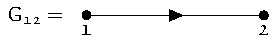
\includegraphics[scale=1.2]{../../Graphics/Diagrams/one_p_green/one_p_green}.
	\caption{Diagrammatic representation of the one-particle Green's function $G_{\mathfrak{12}}$. The electron is annihilated at $\mathfrak{1}$, propagates in imaginary time from $\tau_1$ to $\tau_2$ and is created at $\mathfrak{2}$.}
	\label{fig:one_p_green}
\end{figure}

In homogeneous systems, e.g., infinite or translationally invariant systems, the Green's function inherits the system's properties and becomes invariant under spatial translations. This means that $G_{\mathfrak{12}}(\vv{R}_1, \vv{R}_2)=G_{\mathfrak{12}}(\vv{R}_1-\vv{R}_2,\vv{0})=G_{\mathfrak{12}}(\vv{R})$. In Fourier space, this means that the Green's function is also only dependent on a single momentum parameter, $G_{\mathfrak{12}}(\vv{k}_1, \vv{k}_2)=G_{\mathfrak{12}}(\vv{k}_1-\vv{k}_2,\vv{0})=G_{\mathfrak{12}}(\vv{k})$. Furthermore, if the system is stationary, i.e., the Hamiltonian is not explicitly dependent on imaginary time, then $G_{\mathfrak{12}}(\tau_1, \tau_2)=G_{\mathfrak{12}}(\tau_1-\tau_2,0)=G_{\mathfrak{12}}(\tau)$. In absence of spin-orbit coupling, the spins at $\mathfrak{1}$ and $\mathfrak{2}$ need to be equal and therefore $G_{\mathfrak{12}}$ only depends on a single spin component. Additionally, the \textit{fermionic} Green's function can be shown to be anti-periodic in imaginary time with a period of $\beta$\footnote{This originates from the Boltzmann term $e^{\beta\hat{\mathcal{H}}}$ in the thermal expectation value and restricts the imaginary time domain to $\tau\in[-\beta,\beta)$.},
\begin{subequations}
\begin{align}
	G_{\mathfrak{12}}(\tau)&=-G_{\mathfrak{12}}(\beta-\tau)\quad\text{for } \tau>0 \text{ and}\\
	G_{\mathfrak{12}}(\tau)&=-G_{\mathfrak{12}}(\beta+\tau)\quad\text{for } \tau<0.
\end{align}
\end{subequations}
This anti-periodicity in time leads to the Fourier transform to be defined over a discrete set of imaginary frequencies, the the so-called Matsubara frequencies, which for fermionic quantities are given by $\nu_n=(2n+1)\frac\pi\beta$. In contrast, \textit{bosonic} Green's functions are periodic in imaginary time with period $\beta$ and therefore the Fourier transform includes the set of bosonic Matsubara frequencies $\omega_n=(2n)\frac\pi\beta$. In the following, we will always denote fermionic Matsubara frequencies with $\nu_n$ and bosonic ones with $\omega_n$. The fermionic- and bosonic-like Fourier transforms of $G_{\mathfrak{12}}(\tau)$ become, respectively,
\begin{align}
	G_{\mathfrak{12}}(i\nu_n)=\integral{0}{\beta}{\tau}G_{\mathfrak{12}}(\tau) e^{i\nu_n\tau} \qquad\text{and}\quad G_{\mathfrak{12}}(i\omega_n)=\integral{0}{\beta}{\tau}G_{\mathfrak{12}}(\tau) e^{i\omega_n\tau}
\end{align}
and only require the knowledge of Green's functions for positive imaginary times $\tau$. The inverse Fourier transforms are given by
\begin{align}
	G_{\mathfrak{12}}(\tau)=\frac1\beta \sum_n G_{\mathfrak{12}}(i\nu_n) e^{-i\nu_n\tau} \qquad\text{and}\quad G_{\mathfrak{12}}(\tau)=\frac1\beta \sum_n G_{\mathfrak{12}}(i\omega_n) e^{-i\omega_n\tau}.
\end{align}
If we perform a spectral representation of the fermionic Green's function in \eqref{eq:one_p_green_expectation_val} and calculate the discrete Fourier transform, we find that
\begin{align}
	G_{\mathfrak{12}}(i\nu_n)=\frac1Z\sum_{mn}\left (e^{-\beta E_n}+e^{-\beta E_m}\right )\frac{\sandwich{n}{\hat c_{\mathfrak{1}}}{m}\sandwich{m}{\hat c^{\dagger}_{\mathfrak{2}}}{n}}{i\nu-(E_m-E_n)}.
\end{align}
If we take $\mathfrak{1}\equiv \mathfrak{2}$, which corresponds to the \textit{local} Green's function, we can introduce the spectral function
\begin{align}
	A_{\mathfrak{1}}(\nu)=\frac1Z\sum_{mn} e^{-\beta E_n}\left (1+e^{-\beta\nu}\right ) |\sandwich{n}{\hat c_{\mathfrak{1}}}{m}|^2 \delta(\nu-E_m-E_n),
\end{align}
where,
\begin{align}
	G_{\mathfrak{1}}(i\nu_n)=\integral{\mathbb{R}}{}{\nu}\frac{A_{\mathfrak{1}}(\nu)}{i\nu_n-\nu}.
\end{align}
The spectral function $A_{\mathfrak{1}}(\nu)$ is the probability of adding or removing a particle with momentum $\vv{k}_1$ with spin $\sigma_1$ from the system. For that reason, $A_{\mathfrak{1}}(\nu)$ is coined the single-particle local density of states. Furthermore, since it represents a probability distribution, the integral over all energies of $A_{\mathfrak{1}}(\nu)$ is equal to $1$. It is directly measurable using techniques like angle-resolved photoemission spectroscopy (ARPES), which probes electronic states in the material and reveals electronic structure properties, such as band gaps and quasiparticle dispersions. The peaks in $A_{\mathfrak{1}}(\nu)$ correspond to quasiparticle states, with their position indicating the energy of these states and their width related to the lifetime or decay rate of the quasiparticles. A narrow peak indicates a well-defined quasiparticle with a long lifetime and weak decay rate, while a broad peak suggests the contrary. The spectral function is a key quantity in many-body theory as it connects real-world experimental results to the Green's function formalism, as is shown in the following. By performing analytic continuation in the upper complex plane ($i\nu\to\nu+i0^{+}$), one can define the retarded Green's function as
\begin{align}
	G_{\mathfrak{1}}^{R}(\nu)=\integral{\mathbb{R}}{}{\nu'}\frac{A_{\mathfrak{1}}(\nu')}{\nu-\nu'+i 0^{+}},
\end{align}
from where one obtains through the Kramers-Kronig relations
\begin{align}
	A_{\mathfrak{1}}(\nu) = -\frac1\pi \Im G_{\mathfrak{1}}^{R}(\nu).
\end{align}
Thus, the spectral function is directly coupled to the imaginary part of the retarded Green's function, connecting many-body theory with physical experiments.

As an example, which will prove itself useful for the future, let us consider non-interacting electrons in a system with translational symmetry that are described by the (Wannier) Hamiltonian
\begin{align}
	\hat{\mathcal{H}}_0=\sum_{\vv{k};\mathfrak{12}}\varepsilon_{\mathfrak{12}}(\vv{k})\hat c^{\dagger}_{\vv{k};\mathfrak{1}}\hat c_{\vv{k};\mathfrak{2}},
\end{align}
where $\varepsilon_{\mathfrak{12}}(\vv{k})=-\sum_{\vv{R};\mathfrak{12}} t_{\mathfrak{12}}(\vv{R})e^{i\vv{kR}}$ is the momentum dispersion of the band and is measured with respect to the chemical potential $\mu$. In this case, it is easy to show, that 
\begin{align}\label{eq:non_interacting_one_p_green}
	G_{0;\mathfrak{12}}(\nu_n, \vv{k})=[i\nu_n\delta_{\mathfrak{12}}-\varepsilon_{\mathfrak{12}}(\vv{k})]^{-1}.
\end{align}
For the one-particle spectral function, we find in this case 
\begin{align}
	A_{\mathfrak{12}}(\varepsilon,\vv{k})=\delta(\varepsilon-\varepsilon_{\vv{k};\mathfrak{12}}),
\end{align}
corresponding to stable quasiparticles, due to zero width of the quasiparticle peak of $A_{\mathfrak{12}}(\varepsilon,\vv{k})$.

The direct computation of the Green's function as expressed in \eqref{eq:one_p_green_expectation_val} generally incurs an exponential increase in cost with lattice size for interacting models. As a result, it is common practice to begin with the noninteracting case and construct a perturbative expansion in terms of the interaction around it. In this context, we will start with the non-interacting case described above. This perturbation expansion will not be derived in detail in this thesis, as there are many wonderful resources that explain it very thoroughly \cite{Abrikosov, Nolting}, thus we will only sketch it here. In essence, the expansion is constructed using the so-called $S$-matrix and employs strategies such as the Wick contraction \cite{Wick, evaluation of collision matrix and Notes on wick's theorem} and the linked cluster theorem \cite{linked cluster chapter in book}. The expansion begins by identifying the most general interaction part of the Hamiltonian of \eqref{eq:general_hubbard_hamiltonian},
\begin{align}
	\hat{\mathcal{H}}_{\text{I}} = \frac12 \sum_{\mathfrak{1234}}U_{\mathfrak{1234}}\hat c^{\dagger}_{\mathfrak{1}}\hat c^{\dagger}_{\mathfrak{3}}\hat c_{\mathfrak{4}}\hat c_{\mathfrak{2}}.
\end{align}
The expansion of the Green's function then reads
\begin{align}
	G_{\mathfrak{12}}(\tau)=-\frac{1}{\mean{S(\beta)}_0}\sum_{n=0}^{\infty}\frac{(-1)^n}{n!}\integral{0}{\beta}{\tau_1}\cdots\integral{0}{\beta}{\tau_n}\mean{\mathcal{T}\left [\hat{c}_{\mathfrak{1}}\hat{c}^{\dagger}_{\mathfrak{2}}\hat{\mathcal{H}}_{\text{I}}(\tau_1)\cdots \hat{\mathcal{H}}_{\text{I}}(\tau_n) \right ]}_0,
\end{align}
where $S(\beta)$ is the abovementioned $S$-matrix and $\mean{\cdot}_0$ is the thermal expectation value in terms of the non-interacting Hamiltonian $\hat{\mathcal{H}}_0$. 
In Feynman diagram jargon, this contains all diagrams that are possible, also disconnected ones\footnote{Disconnected means, that the term includes a diagram that consists of two separate, disconnected diagrams.}. The linked cluster theorem allows us to get rid of those disconnected contributions by effectively cancelling with the $\frac{1}{\mean{S(\beta)}_0}$ term in front. This results in
\begin{align}\label{eq:one_p_green_full_perturbation_exp}
	G_{\mathfrak{12}}(\tau)=-\sum_{n=0}^{\infty}\frac{(-1)^n}{n!}\integral{0}{\beta}{\tau_1}\cdots\integral{0}{\beta}{\tau_n}\mean{\mathcal{T}\left [\hat{c}_{\mathfrak{1}}\hat{c}^{\dagger}_{\mathfrak{2}}\hat{\mathcal{H}}_{\text{I}}(\tau_1)\cdots \hat{\mathcal{H}}_{\text{I}}(\tau_n) \right ]}_0^{\text{conn}},
\end{align}
where $\mean{\cdot}_0^{\text{conn}}$ now indicates that we only consider connected diagrams in the expansion. We can transform this into a diagrammatic representation by applying Wick contractions, which allow us to collect pairs of creation and annihilation operators to form independent expectation values. In the case of the $n=1$ term in the perturbation expansion of the Green's function,
\begin{align}
\begin{split}
	G_{1;\mathfrak{12}}(\tau)=\sum_{\mathfrak{abcd}}\integral{0}{\beta}{\tau_1}U_{\mathfrak{abcd}}\bigg[&- \mean{\mathcal{T}\left [\hat{c}_{\mathfrak{1}}(\tau)\hat{c}^{\dagger}_{\mathfrak{a}}(\tau_1)\right ]}_0 \mean{\mathcal{T}\left [\hat{c}_{\mathfrak{d}}(\tau_1)\hat{c}^{\dagger}_{\mathfrak{c}}(\tau_1)\right ]}_0 \mean{\mathcal{T}\left [\hat{c}_{\mathfrak{b}}(\tau_1)\hat{c}^{\dagger}_{\mathfrak{2}}(0)\right ]}_0\\
	&+\mean{\mathcal{T}\left [\hat{c}_{\mathfrak{1}}(\tau)\hat{c}^{\dagger}_{\mathfrak{a}}(\tau_1)\right ]}_0 \mean{\mathcal{T}\left [\hat{c}_{\mathfrak{b}}(\tau_1)\hat{c}^{\dagger}_{\mathfrak{c}}(\tau_1)\right ]}_0 \mean{\mathcal{T}\left [\hat{c}_{\mathfrak{d}}(\tau_1)\hat{c}^{\dagger}_{\mathfrak{2}}(0)\right ]}_0\bigg].
\end{split}
\end{align}
The remaining expectation values are nothing more than minus the non-interacting Green's function of \eqref{eq:non_interacting_one_p_green}. Written in Feynman diagrams, the first relevant perturbation expansion term is shown in \figref{fig:one_p_green_first_perturbation_term}.
\begin{figure}[ht!]
	\centering
	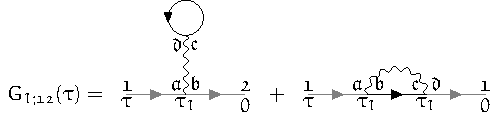
\includegraphics[scale=1.2]{../../Graphics/Diagrams/one_p_green_first_perturbation_term/one_p_green_first_perturbation_term}
	\caption{First order diagrams for the single-particle Green's function. The corresponding diagrams are coined the Hartree- and the Fock-term, respectively. As the name suggests, taking only these two diagrams as the whole perturbation expansion leads to the Hartree-Fock approximation, formulated as a diagrammatic theory.}
	\label{fig:one_p_green_first_perturbation_term}
\end{figure}

\section{Self-energy}

The one-particle Green's function perturbative expansion is already much simplified in the graphical portrayal. However, the number of diagrams increases exponentially with order $n$\footnote{For $n=2$ there exist $10$ diagrams, for $n=7$ the number of diagrams is well over a million.}. Therefore, the Feynman diagram approach would be of little practical use if the only way to progress was to calculate each diagram one at a time. However, in reality the technique is actually quite useful, since it hints on how to sum up the perturbative series. Let us talk about how it applies to Green's function for single particles. First, let us define another compound index which will further levitate readability. We will set $\k=\{\nu,\vv{k}\}$ and $\q=\{\omega, \vv{q}\}$ as a compound index including momentum and frequency in one index for fermionic ($\k$) and bosonic ($\q$) frequencies and momenta. Note, that if we write $\nu$ instead of $\k$, we refer to the \textit{local} part of the quantity with $\vv{k}=\vv{0}$ instead of the \textit{non-local} part.

Diagrams in general can be split up into two classes: (i) diagrams that, by cutting a single internal Green's function line, transform in two lower-order diagrams, which are called one-particle reducible and (ii) diagrams that are not one-particle reducible, which are called one-particle irreducible (1PI). Let us define as the one-particle self-energy $\Sigma_{\mathfrak{12}}^{\k}$ the sum of all irreducible diagrams without external legs. For example, the black part of the diagrams in \figref{fig:one_p_green_first_perturbation_term} corresponds to the first-order diagrams of the self-energy. It is then straightforward to rewrite \eqref{eq:one_p_green_full_perturbation_exp} in terms of the self-energy, yielding
\begin{align}\label{eq:dyson_eq}
	G_{\mathfrak{12}}^{\k}=G_{0,\mathfrak{12}}^{\k}+\sum_{\mathfrak{ab}}G_{0,\mathfrak{1a}}^{\k}\Sigma_{\mathfrak{ab}}^{\k}G_{\mathfrak{b2}}^{\k},
\end{align}
which results in - when taking \eqref{eq:non_interacting_one_p_green} as the noninteracting Green's function and inverting in frequency and momentum space - a way to express the full (interacting) single-particle Green's function in terms of the self-energy
\begin{align}
	G_{\mathfrak{12}}^{\k} = \left [i\nu_n\delta_{\mathfrak{12}}-\varepsilon_{\mathfrak{12}}(\vv{k})-\Sigma_{\mathfrak{12}}^{\k}\right ]^{-1}.
\end{align}
\eqref{eq:dyson_eq} is commonly known as the Dyson equation \cite{dyson eq} for the single-particle Green's function and for completeness, its diagrammatic representation can be found in \figref{fig:dyson_eq}. It is a geometric series, where each term in the sum subsequently adds irreducible diagrams that are pieced together by non-interacting Green's functions to generate all possible diagrams.
\begin{figure}[ht!]
	\centering
	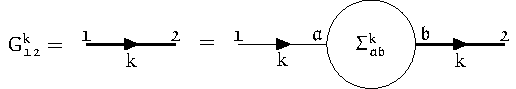
\includegraphics[scale=1.2]{../../Graphics/Diagrams/dyson_eq/dyson_eq}
	\caption{Diagrammatic representation of \eqref{eq:dyson_eq}. The full Green's function $G_{\mathfrak{12}}^{\k}$ is drawn as a thick black line.}
	\label{fig:dyson_eq}
\end{figure}
The self-energy can be obtained by simply inverting \eqref{eq:dyson_eq},
\begin{align}
	\Sigma_{\mathfrak{12}}^{\k}=(G_{0;\mathfrak{12}}^{\k})^{-1}-(G_{\mathfrak{12}}^{\k})^{-1}.
\end{align}
Thus, perturbation theory can be done in two distinct ways: the simpler approach is to determine the Green's function directly, for example, up to order $n$, where the second method is to compute the self-energy up to order $n$ and insert its expression in the Dyson equation \eqref{eq:dyson_eq}. This gives an approximate Green's function containing each order of perturbation theory with only a subset of all possible diagrams. As a result, \eqref{eq:dyson_eq} represents a way to sum up perturbation theory and is actually more relevant from a physical standpoint. Indeed, many methods leverage the usefulness of this approach, for example the dynamical mean-field theory or the dynamical vertex approximation, as we will see later.

Let us add some physical background to the self-energy in the following. $\Sigma$ represents the effects of the interaction on the single electron propagators. The real and imaginary part of the self-energy have significant impact on the physical properties of the system. The real part of the self-energy contributes to an energy shift of the electronic states of the single-particle energy levels $\epsilon(\vv{k})$ due to interactions. In contrast, the imaginary part of the self-energy is related to the decay or lifetime of quasiparticles and introduces a spectral broadening or damping of the electronic states, indicating how long an excitation or quasiparticle persists before interacting with other excitations or scattering events. A larger imaginary part implies a shorter lifetime and stronger interactions. The first order derivative in frequency, $\dpd{\Sigma^{\k}}{\nu}$, contributes to an effective renormalization of the bare electron mass. It also leads to a redistribution of spectral weight in the one-particle spectral function, which provides information about the distribution of energy levels available for excitations. A broader spectral function, whose broadening is controlled by the imaginary part of the self-energy, typically indicates stronger interactions and a more correlated system.

\section{Two-particle Green's functions}

In analogy to the one-particle Green's function, the two-particle Green's function describes the amplitude of the propagation of two particles, two holes or a particle and a hole. A similar expression to \eqref{fig:one_p_green} can be formulated for the two-particle Green's function
\begin{align}
	G_{\mathfrak{1234}}^{\q\k\kp}=-\mean{\mathcal{T}\left [\hat{c}_{\vv{k};\mathfrak{1}}\hat{c}^{\dagger}_{\vv{k}-\vv{q};\mathfrak{2}}\hat{c}_{\vv{k}'-\vv{q};\mathfrak{3}}\hat{c}^{\dagger}_{\vv{k}';\mathfrak{4}}\right ]}.
\end{align}
It describes two particles, two holes or a particle and a hole being inserted in the system at times $\tau_2$ and $\tau_4$, propagating in the system until they are removed again at $\tau_1$ and $\tau_3$, respectively. Assuming a stationary Hamiltonian that satisfies time-translation invariance, it is possible to eliminate one imaginary time variable by setting it zero. Then, the Green's function only depends on three time variables and through Fourier transform, also only depends on three frequency and momentum variables. 
Furthermore, similar to the case for the one-particle Green's function, the absence of spin-orbit coupling reduces the number of spin degrees of freedom 
\begin{subequations}
\begin{align}
	G_{\sigma\sigma';\mathfrak{1234}}^{\q\k\kp}&=G_{\sigma\sigma\sigma'\sigma';\mathfrak{1234}}^{\q\k\kp} \qquad\text{and}\\
	G_{\overline{\sigma\sigma'};\mathfrak{1234}}^{\q\k\kp}&=G_{\sigma\sigma'\sigma'\sigma;\mathfrak{1234}}^{\q\k\kp}.
\end{align}
\end{subequations}
In this case, the total incoming and outgoing spin must be equal and this puts a heavy constraint on the possible spin combinations,
\begin{align}
	\sigma_1=\sigma_2=\sigma_3=\sigma_4, \qquad (\sigma_1=\sigma_2) \neq (\sigma_3=\sigma_4)\qquad\text{and}\qquad (\sigma_1=\sigma_4)\neq(\sigma_2=\sigma_3),
\end{align}
totaling to only six unique spin combinations, each of which can be seen in \figref{fig:two_particle_green_spins}.
\begin{figure}[h]
  \centering
  \subfloat{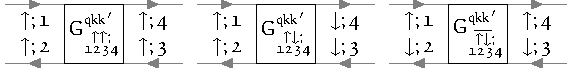
\includegraphics[scale=1.2]{../../Graphics/Diagrams/two_particle_green_spins/two_particle_green_spins_row1}}\vspace{0.5cm}\\
  \subfloat{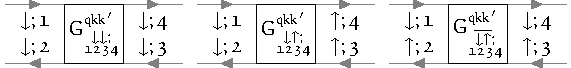
\includegraphics[scale=1.2]{../../Graphics/Diagrams/two_particle_green_spins/two_particle_green_spins_row2}}
  \caption{In the case of absent spin-orbit coupling, these are the only non-vanishing spin combinations of the two-particle Green's function.}
  \label{fig:two_particle_green_spins}
\end{figure}
Furthermore, if one describes quantities in the paramagnetic phase, where the system is SU(2)-symmetric, there are only two independent spin configurations,
\begin{subequations}
\begin{align}
	G_{\sigma\sigma';\mathfrak{1234}}^{\q\k\kp}&=G_{(-\sigma)(-\sigma');\mathfrak{1234}}^{\q\k\kp}=G_{\sigma'\sigma;\mathfrak{1234}}^{\q\k\kp}\qquad\text{and}\\
	G_{\sigma\sigma;\mathfrak{1234}}^{\q\k\kp}&=G_{\sigma(-\sigma);\mathfrak{1234}}^{\q\k\kp}+G_{\overline{\sigma(-\sigma)};\mathfrak{1234}}^{\q\k\kp}.
\end{align}
\end{subequations}
For these two spin combinations, the density and magnetic channel specified in the following are a particularly helpful choice of notation, as we shall see in the upcoming sections: 
\begin{subequations}
\begin{align}
	G_{\text{d};\mathfrak{1234}}^{\q\k\kp}&=G_{\uparrow\uparrow;\mathfrak{1234}}^{\q\k\kp}+G_{\uparrow\downarrow;\mathfrak{1234}}^{\q\k\kp}\qquad\text{and}\label{eq:two_particle_green_density}\\
	G_{\text{m};\mathfrak{1234}}^{\q\k\kp}&=G_{\uparrow\uparrow;\mathfrak{1234}}^{\q\k\kp}-G_{\uparrow\downarrow;\mathfrak{1234}}^{\q\k\kp}=G_{\overline{\uparrow\downarrow};\mathfrak{1234}}^{\q\k\kp}.\label{eq:two_particle_green_magnetic}
\end{align}
\end{subequations}
Besides the spin-symmetries discussed above, the Green's function also inherits other properties of the system, such as time-reversal symmetry, which manifests itself by
\begin{align}
	G_{\mathfrak{1234}}^{\q\k\kp}=G_{\mathfrak{3421}}^{\bar\q\bar{\text{k}}'\bar\k},
\end{align} 
where $\overline\k=\{\nu,-\vv{k}\}$ is the time-reversed compound momentum variable. Furthermore, the two-particle Green's function satisfies the crossing symmetry, which is a direct manifestation of Pauli's principle. Crossing symmetry refers to the antisymmetric property of the Green's function with respect to the exchange of the incoming and outgoing fermions
\begin{subequations}
\begin{align}
	G_{\sigma\sigma';\mathfrak{1234}}^{\q\k\kp}&= -G_{\overline{\sigma'\sigma};\mathfrak{3214}}^{(\kp-\k)(\kp-\q)\kp}\label{eq:crossing_sym_1}\\
	&= -G_{\overline{\sigma\sigma'};\mathfrak{1432}}^{(\k-\kp)\k(\k-\q)}\label{eq:crossing_sym_2}\\
	&= G_{\sigma'\sigma;\mathfrak{3412}}^{(-\q)(\kp-\q)(\k-\q)}.\label{eq:crossing_sym_3}
\end{align}
\end{subequations}
The symmetries \eqref{eq:crossing_sym_1} - \eqref{eq:crossing_sym_3} describe the frequency changes that occur by exchanging the positions of the gray fermion lines, leaving the vertex unchanged. The last line corresponds to a full swap of the incoming and outgoing particle labels. The crossing symmetry is visually shown in \figref{fig:two_particle_green_crossing_symmetry}. Lastly, the Green's function also possesses symmetry with respect to complex conjugation,
\begin{align}
	\left (G_{\sigma\sigma';\mathfrak{1234}}^{\q\k\kp}\right )^*=G_{\sigma'\sigma;\mathfrak{4321}}^{(-\q)(-\k)(-\kp)}.
\end{align}
\begin{figure}[h]
  \centering
  \subfloat{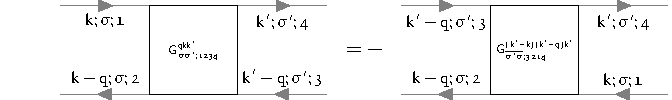
\includegraphics[scale=1.4]{../../Graphics/Diagrams/two_particle_green_crossing_symmetry/two_particle_green_crossing_symmetry_row1}}\vspace{0.5cm}\\
  \subfloat{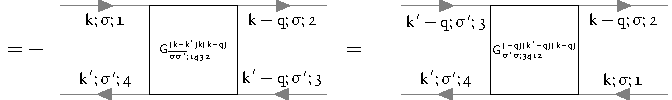
\includegraphics[scale=1.4]{../../Graphics/Diagrams/two_particle_green_crossing_symmetry/two_particle_green_crossing_symmetry_row2}}
  \caption{Diagrammatic representation of the crossing symmetry relations in order of \eqref{eq:crossing_sym_1} - \eqref{eq:crossing_sym_3}.}
  \label{fig:two_particle_green_crossing_symmetry}
\end{figure}
At the beginning of the section it was stated that the (four-point) two-particle Green's function only requires three frequency arguments to be fixed since the last one is automatically given by momentum conservation. There are three equivalent choices (coined channels) of independent frequencies (with $\nu$, $\nu'$ being a fermionic and $\omega$ a bosonic Matsubara frequency)
\begin{subequations}
\begin{align}
	\text{ph-notation:}&\;\;\{\nu_1=\nu,&&\nu_2=\nu-\omega,&&\nu_3=\nu'-\omega,&&\nu_4=\nu'\},\label{eq:ph_freq}\\
	\overline{\text{ph}}\text{-notation:}&\;\;\{\nu_1=\nu,&&\nu_2=\nu',&&\nu_3=\nu'-\omega,&&\nu_4=\nu-\omega\}\qquad\text{and}\label{eq:ph_bar_freq}\\
	\text{pp-notation:}&\;\;\{\nu_1=\nu,&&\nu_2=\omega-\nu',&&\nu_3=\omega-\nu,&&\nu_4=\nu'\}.\label{eq:pp_freq}
\end{align}
\end{subequations}
To show the effects of this frequency shift and how they affect the labels of the diagrams, we show the two-particle Green's function in the three notations of \eqref{eq:ph_freq} - \eqref{eq:pp_freq} in \figref{fig:two_particle_green_channels} below.
\begin{figure}[h]
  \centering
  \subfloat{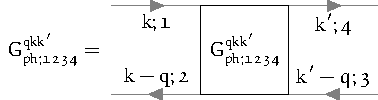
\includegraphics[scale=1.2]{../../Graphics/Diagrams/two_particle_green_channels/two_particle_green_channels_ph}}\vspace{0.5cm}\\
  \subfloat{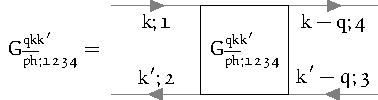
\includegraphics[scale=1.2]{../../Graphics/Diagrams/two_particle_green_channels/two_particle_green_channels_ph_bar}}\vspace{0.5cm}\\
  \subfloat{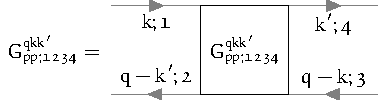
\includegraphics[scale=1.2]{../../Graphics/Diagrams/two_particle_green_channels/two_particle_green_channels_pp}}
  \caption{Two-particle Green's functions in the different frequency notations of \eqref{eq:ph_freq} - \eqref{eq:pp_freq} expressed in Feynman diagrams. The frequency notation is encoded in an additional subscript, $\{\text{ph}, \overline{\text{ph}},\text{pp}\}$.}
  \label{fig:two_particle_green_channels}
\end{figure}
Obviously, the choice of frequency convention should not have any impact on the physical content of the Green's function, hence it is possible to switch between these channels by applying channel-specific frequency shifts,
\begin{subequations}
\begin{align}
	G_{\text{ph};\mathfrak{1234}}^{\q\k\kp}&=G_{\overline{\text{ph}};\mathfrak{1234}}^{(\k-\kp)\k(\k-\q)},\\
	G_{\overline{\text{ph}};\mathfrak{1234}}^{\q\k\kp}&=G_{\text{ph};\mathfrak{1234}}^{(\k-\kp)\k(\k-\q)},\\
	G_{\text{ph};\mathfrak{1234}}^{\q\k\kp}&=G_{\text{pp};\mathfrak{1234}}^{(\k+\kp-\q)\k\kp}\qquad\text{and}\\
	G_{\text{pp};\mathfrak{1234}}^{\q\k\kp}&=G_{\text{ph};\mathfrak{1234}}^{(\k+\kp-\q)\k\kp}.
\end{align}
\end{subequations}
Let us finally note that the two-particle Green's function represents all diagrams that are possible that involve two electrons, two holes or an electron and a hole. It can therefore be split into two parts: (i) a part, where the electrons do not interact with each other and propagate independently; and (ii) a part, where the electrons do interact with each other through an infinite number of processes. (ii) is commonly called the connected two-particle Green's function and can be mathematically formulated by
\begin{align}\label{eq:two_particle_green_connected}
	G_{\sigma\sigma';\mathfrak{1234}}^{\q\k\kp}=G_{\sigma\sigma';\mathfrak{1234}}^{\text{conn};\q\k\kp}+\delta_{\q0}G_{\sigma;\mathfrak{12}}^{\k}G_{\sigma';\mathfrak{34}}^{\kp}-\delta_{\sigma\sigma'}\delta_{\k\kp}G_{\sigma;\mathfrak{14}}^{\k}G_{\sigma;\mathfrak{32}}^{\k-\q}.
\end{align}
Diagrammatically, the connected two-particle Green's function contains all diagrams, where two propagating electrons interact with each other. The first terms up to interaction order two are given in \figref{fig:two_particle_green_connected}.
\begin{figure}[h]
  \centering
  \subfloat{\includestandalone[width=\textwidth]{../../Graphics/Diagrams/two_particle_green_connected/two_particle_green_connected_separate_row1}}\vspace{0.5cm}\\
  \subfloat{\includestandalone[width=\textwidth]{../../Graphics/Diagrams/two_particle_green_connected/two_particle_green_connected_separate_row2}}\vspace{0.5cm}\\
  \subfloat{\includestandalone[width=\textwidth]{../../Graphics/Diagrams/two_particle_green_connected/two_particle_green_connected_separate_row3}}
  \caption{Diagrammatic representation of the two-particle connected Green's function up to order two. It includes the possible interaction processes that occur between two propagating electrons. The particle labels are only written down for the first diagram, the other diagrams are labeled analogously.}
  \label{fig:two_particle_green_connected}
\end{figure}
The other terms in \eqref{eq:two_particle_green_connected} are not that interesting, they merely describe the electrons propagating in the system without ever interacting with the other. However, we will still show the diagrammatic content of the second and third term of \eqref{eq:two_particle_green_connected} in \figref{fig:two_particle_green_disconnected}.
\begin{figure}[ht!]
	\centering
	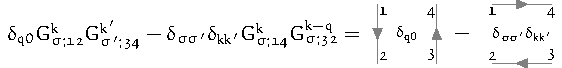
\includegraphics[scale=1.2]{../../Graphics/Diagrams/two_particle_green_disconnected/two_particle_green_disconnected}
	\caption{Disconnected part (second and third term on the right hand side of \eqref{eq:two_particle_green_connected}) of the two-particle Green's function.}
	\label{fig:two_particle_green_disconnected}
\end{figure}
The connected two-particle Green's function without the external legs is commonly called the full vertex $F$, where by convention an additional minus sign is introduced,
\begin{align}
	G_{\mathfrak{1234}}^{\text{conn};\q\k\kp} = -\frac1\beta \sum_{\mathfrak{abcd}} G_{\mathfrak{1a}}^{\k} G_{\mathfrak{b2}}^{\k-q} F_{\mathfrak{1234}}^{\q\k\kp} G_{\mathfrak{3c}}^{\kp-q} G_{\mathfrak{d4}}^{\kp}.
\end{align}
By the previous definition, the vertex function $F_{\mathfrak{1234}}^{\q\k\kp}$ contains all diagrams that connect two incoming and two outgoing lines. All diagrams contained in the full vertex $F_{\mathfrak{1234}}^{\q\k\kp}$ can be classified by their two-particle reducibility (2PR). A diagram is called two-particle reducible, if it can be split into two separate parts by cutting two internal Green's function lines. Furthermore, this classification is described by three channels, $\{\text{ph},\overline{\text{ph}},\text{pp}\}$, depending on which incoming and outgoing lines are being separated by the \say{cutting}-process. The $\text{ph}$-channel corresponds to those diagrams, where the sub-parts connect $\mathfrak{12}$ and $\mathfrak{34}$, for the $\overline{\text{ph}}$-channel $\mathfrak{14}$ and $\mathfrak{23}$ and for the $\text{pp}$-channel $\mathfrak{13}$ and $\mathfrak{24}$ are connected. These reducible diagrams are categorized in $\Phi_{\text{ph};\mathfrak{1234}}^{\q\k\kp}$, $\Phi_{\overline{\text{ph}};\mathfrak{1234}}^{\q\k\kp}$ and $\Phi_{\text{pp};\mathfrak{1234}}^{\q\k\kp}$, respectively. All diagrams that are not two-particle reducible are grouped together in the quantity $\Lambda_{\mathfrak{1234}}^{\q\k\kp}$. This procedure is called the Parquet-decomposition and reads mathematically
\begin{align}\label{eq:parquet_decomposition}
	F_{\mathfrak{1234}}^{\q\k\kp}=\Lambda_{\mathfrak{1234}}^{\q\k\kp}+\Phi_{\text{ph};\mathfrak{1234}}^{\q\k\kp}+\Phi_{\overline{\text{ph}};\mathfrak{1234}}^{\q\k\kp}+\Phi_{\text{pp};\mathfrak{1234}}^{\q\k\kp}.
\end{align}
Another possibility is to split up the full vertex $F$ in reducible and irreducible diagrams in a specific channel $\text{r}\in\{\text{ph},\overline{\text{ph}},\text{pp}\}$,
\begin{align}\label{eq:full_vertex_gamma_phi}
	F_{\mathfrak{1234}}^{\q\k\kp}=\Gamma_{\text{r};\mathfrak{1234}}^{\q\k\kp}+\Phi_{\text{r};\mathfrak{1234}}^{\q\k\kp},
\end{align}
where $\Gamma_{\text{r};\mathfrak{1234}}^{\q\k\kp}$ is the irreducible vertex in channel $\text{r}$ and $\Phi_{\text{r};\mathfrak{1234}}^{\q\k\kp}$ the corresponding reducible one. Note, that in channel $\text{r}$ irreducible diagrams might still be reducible in another channel $\text{r}'\neq \text{r}$. For example, $\Gamma_{\text{ph};\mathfrak{1234}}^{\q\k\kp}$ contains all fully irreducible diagrams, but also all diagrams which are reducible in channels $\overline{\text{ph}}$ and $\text{pp}$,
\begin{align}
	\Gamma_{\text{ph};\mathfrak{1234}}^{\q\k\kp}=\Lambda_{\mathfrak{1234}}^{\q\k\kp}+\Phi_{\overline{\text{ph}};\mathfrak{1234}}^{\q\k\kp}+\Phi_{\text{pp};\mathfrak{1234}}^{\q\k\kp}.
\end{align}
This will be important later in \secref{sec:bethe_salpeter}, where we will discuss the Bethe-Salpeter equations. Before that, let us briefly introduce the concept of linear response and the central physical property describing the response of a system with respect to an external perturbation\footnote{For example an external electromagnetic field.}, the susceptibility.

\section{Susceptibility}

Experimentally, it is not possible to directly extract information (just by \say{looking}) about the interactions between electrons in a system. Instead, in spectroscopic experiments, a perturbation is applied to the system and one measures the system's response. In particular, one measures how expectation values $\mean{\cdot}$ of operators (take the multi-dimensional operator $\hat O_{i}(\tau)$ as an example) changes when an external field $h_{j}(\tau)$ is applied. In linear response theory, this response is - as the name suggests - taken to be linear in the perturbing field, requiring this field to be sufficiently small in order for this description to be a good approximation,
\begin{align}
	\mean{\hat O_{i}(\tau)}_{\vv{h}}-\mean{\hat O_{i}(\tau)}_{\vv{h}=0}=\integral{0}{\beta}{\tau'} \chi_{ij}(\tau-\tau')h_{j}(\tau')+\mathcal{O}(\vv{h}^2),
\end{align}
where $\chi_{ij}(\tau-\tau')$ is coined physical susceptibility and does not depend on the field $h_{j}(\tau)$. $\chi(\tau-\tau')$ fulfills the Kramers-Kronig relations, is causal ($\chi_{ij}(\tau-\tau')=\Theta(\tau-\tau')\chi_{ij}(\tau-\tau')$) and is finite ($\forall\, \tau,\tau':\;\exists\, C\in\mathbb{R}:\; |\chi_{ij}(\tau-\tau')|<C$). The susceptibility can be computed straightforwardly by taking the functional derivative of $\hat O_{i}(\tau)$ with respect to the field $h_{j}(\tau)$,
\begin{align}
	\chi_{ij}(\tau-\tau')=\ddd{\mean{\hat O_{i}(\tau')}}{h_{j}(\tau)}\bigg|_{\vv{h}=0}=\mean{\mathcal{T}\hat O_{i}(\tau)\hat O_{j}(\tau')}-\mean{\hat O_{i}}\mean{\hat O_{j}}.
\end{align}
On the two-particle level, only the density's response to variations in the one-particle energy, $\chi_{\text{d}}$, and the magnetization's response to variation in the electromagnetic field in the same direction, $\chi_{\text{m}}$, are non-zero
\begin{subequations}
\begin{align}
	\chi_{\text{d}}(\tau)&=\chi_{nn}(\tau)=-\ddd{\mean{\hat n}}{\mu(\tau)}\bigg|_{\mu=0}\qquad\text{and}\label{eq:chi_dens_derivative}\\
	\chi_{\text{m}}(\tau)&=\chi_{ii}(\tau)=\ddd{\mean{\hat\sigma_{i}}}{h_{i}(\tau)}\bigg|_{\vv{h}=0},\label{eq:chi_magn_derivative}
\end{align}
\end{subequations}
where $i\in\{x,y,z\}$. The physical susceptibilities are included in the two-particle Green's function, as we will see shortly. In fact, the sum of terms corresponding to the two disconnected, horizontal Green's function lines and the vertex part is denoted as the general susceptibility and can be expressed as
\begin{align*}\label{eq:generalized susceptibility}
	\chi_{\mathfrak{1234}}^{\q\k\kp}&=\beta\left (G_{\mathfrak{1234}}^{\q\k\kp}-\delta_{q0}G_{\mathfrak{12}}^{\k} G_{\mathfrak{34}}^{\kp}\right )\\
	&=-\beta\delta_{\k\kp}G_{\mathfrak{14}}^{\k}G_{\mathfrak{32}}^{\k-\q}-\sum_{\mathfrak{abcd}} G_{\mathfrak{1a}}^{\k} G_{\mathfrak{b2}}^{\k-q} F_{\mathfrak{abcd}}^{\q\k\kp} G_{\mathfrak{3c}}^{\kp-q} G_{\mathfrak{d4}}^{\kp}\\
	&=\chi_{0;\mathfrak{1234}}^{\q\k\k}-\frac{1}{\beta^2}\sum_{\mathfrak{abcd}}\chi_{0;\mathfrak{12ba}}^{\q\k\k} F_{\mathfrak{abcd}}^{\q\k\kp} \chi_{0;\mathfrak{dc34}}^{\q\kp\kp},\numberthis
\end{align*}
where
\begin{align}
	\chi_{0;\mathfrak{1234}}^{\q\k\kp}=-\beta G_{\mathfrak{14}}^{\k}G_{\mathfrak{32}}^{\kp-\q}
\end{align}
is commonly denoted as the generalized bubble susceptibility. From this one can obtain physical susceptibilities by contracting the inner legs, i.e.,
\begin{align}\label{eq:phys_susc_contracted_legs}
	\chi_{\mathfrak{14}}^{\q}=\sum_{\k\kp;\mathfrak{23}}\chi_{\mathfrak{1234}}^{\q\k\kp}.
\end{align}
The diagrammatic content of the physical susceptibility is shown in \figref{fig:physical_susceptibility} below.
\begin{figure}[ht!]
	\centering
	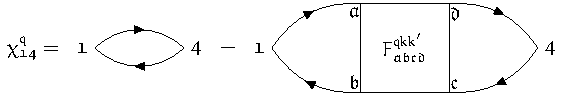
\includegraphics[scale=1.2]{../../Graphics/Diagrams/physical_susceptibility/physical_susceptibility}
	\caption{The physical susceptibility is equal to the generalized susceptibility with contracted legs, see \eqref{eq:phys_susc_contracted_legs}.}
	\label{fig:physical_susceptibility}
\end{figure}
Similarly, the contracted bubble susceptibility can be written as
\begin{align}
	\chi_{0;\mathfrak{14}}^{\q}=\sum_{\k\kp;\mathfrak{23}}\chi_{0;\mathfrak{1234}}^{\q\k\kp}.
\end{align}
Similarly to \eqref{eq:two_particle_green_density} and \eqref{eq:two_particle_green_magnetic}, one can write down density and magnetic spin combinations,
\begin{subequations}
\begin{align}
	\chi_{\text{d}}^{\q}&=\chi_{\uparrow\uparrow}^{\q}+\chi_{\uparrow\downarrow}^{\q}=\chi_{\overline{\uparrow\downarrow}}^{\q}\qquad\text{and}\label{eq:chi_dens}\\
	\chi_{\text{m}}^{\q}&=\chi_{\uparrow\uparrow}^{\q}+\chi_{\uparrow\downarrow}^{\q}.\label{eq:chi_magn}
\end{align}
\end{subequations}
Note that expressions \eqref{eq:chi_dens} and \eqref{eq:chi_magn} are nothing more than the Fourier transformed versions of \eqref{eq:chi_dens_derivative} and \eqref{eq:chi_magn_derivative}, respectively.

\section{Vertex asymptotics}

A full treatment of frequency and momentum dependence of multi-orbital vertex functions severely restricts the speed and memory consumption of numerical calculations. A step towards reducing the computational cost of numerical implementations of equations involving vertex functions, such as the Bethe-Salpeter equations, see \secref{sec:bethe_salpeter}, or the Schwinger-Dyson equation, see \secref{sec:schwinger_dyson}, thus requires an efficient treatment of the vertex for high Matsubara frequencies. We will see that the vertex - in the high-frequency regime - which originally depended on three independent frequency parameters can be treated as an object with only two frequency dimensions, thus drastically reducing the storage capacity of and ease of calculations including the vertex.
\begin{figure}[ht!]
	\centering
	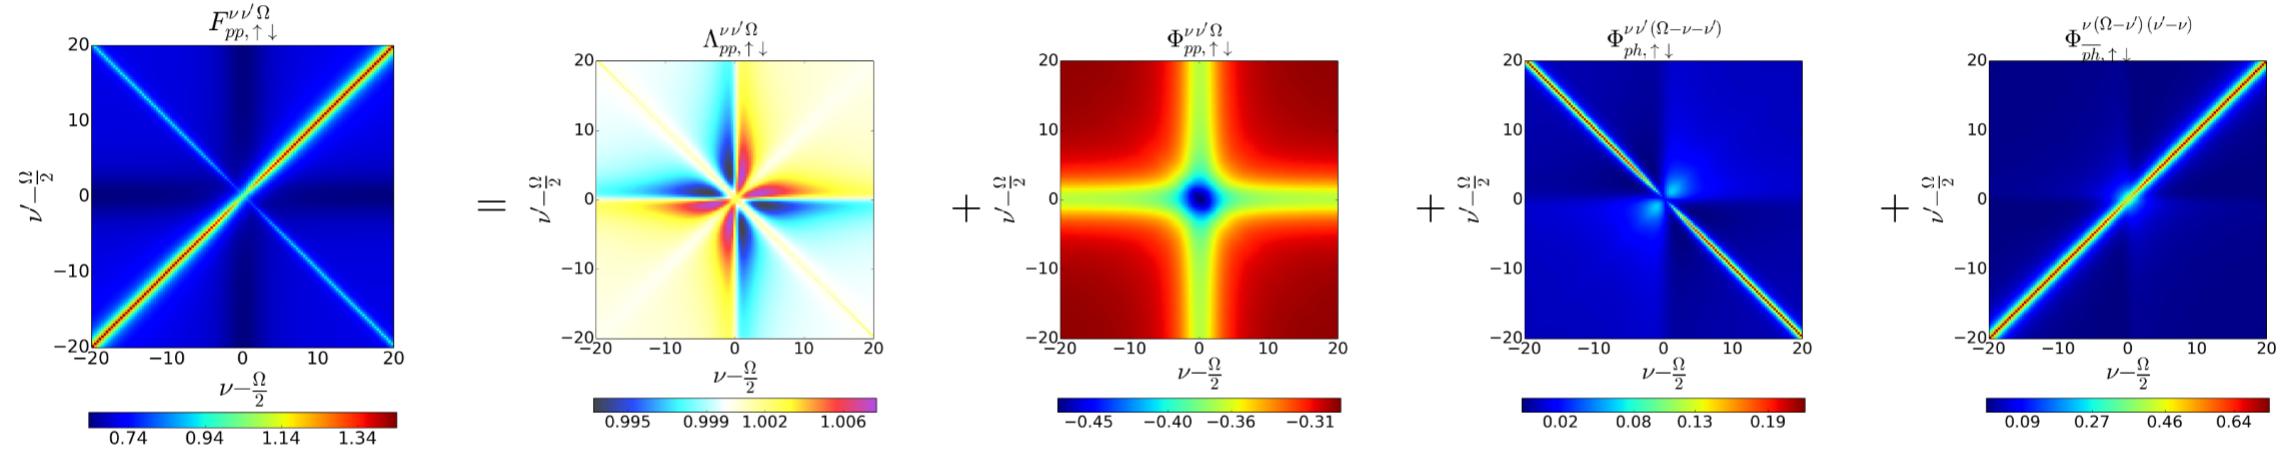
\includegraphics[width=\linewidth]{../../Graphics/vertex_asymptotics_paper.png}
	\caption{Numerical SIAM results for all local vertices contained in the Parquet equation \eqref{eq:parquet_decomposition} for vanishing transfer frequency $\Omega=0$, taken from Ref. \cite{high-freq asympt}. In our convention, $\Omega$ should be replaced by $\omega$.}
	\label{fig:full_vertex_siam_results_paper}
\end{figure}
In \figref{fig:full_vertex_siam_results_paper}, the frequency dependence of local vertex functions $F^{\omega\nu\nu'}_{\text{pp};\uparrow\downarrow}$, $\Lambda^{\omega\nu\nu'}_{\text{pp};\uparrow\downarrow}$ and $\Phi^{\omega\nu\nu'}_{\text{r};\uparrow\downarrow}$ calculated for the Single-Impurity Anderson Model (SIAM) are shown for vanishing transfer frequency $\omega$ \cite{high-freq asympt}. From this, one can see three very prominent and distinct features of the full vertex $F$: (i) a constant background that differs from the (local and constant) Hubbard interaction $U$; (ii) two diagonal structures, the main ($\nu=\nu'$) and secondary ($\nu=-\nu'$) diagonal; and (iii) a \say{cross}-like structure along $\nu=\pm\frac\pi\beta$ and $\nu'=\pm\frac\pi\beta$. While only shown for the antiparallel spin combination $\uparrow\downarrow$ and vanishing transfer frequency $\omega=0$, the features are analogous for the parallel spin combination $\uparrow\uparrow$ and for finite $\omega$. These three attributes do \textit{not} decay for high Matsubara frequencies $\nu$ and $\nu'$ and therefore indicate complex asymptotic behaviour. The individual asymptotic contributions of the fully irreducible vertex $\Lambda$ and the reducible vertex in channel r to the full vertex $F$ are written in detail in Ref. \cite{high-freq asympt}. Summarized, $\Lambda$ adds a constant background of size $U$, $\Phi_{\text{ph}}$ adds a secondary diagonal structure, $\Phi_{\overline{\text{ph}}}$ adds a diagonal structure and $\Phi_{\text{pp}}$ adds a constant background and a \say{cross}-like structure. Notice that the description in Ref. \cite{high-freq asympt} only refers to the SIAM model and considers solely the one-band case with local quantities and a constant local interaction $U$. An extension to a multi-orbital formalism and momentum-dependent vertices and interaction $U$ follows naturally and will be discussed shortly.

The simplest quantity to describe in terms of their asymptotics is the fully irreducible vertex $\Lambda^{\q\k\kp}_{\mathfrak{1234}}$, for which
\begin{align}
	\Lambda^{\text{asympt};\q\k\kp}_{\text{ph};\mathfrak{1234};\sigma\sigma'}\approx\mathcal{U}^{\textbf{qkk}'}_{\text{ph};\mathfrak{1234};\sigma\sigma'},
\end{align}
where $\mathcal{U}^{\textbf{qkk}'}_{\mathfrak{1234};\sigma\sigma'}$ is the non-local Coulomb interaction, written in crossing-symmetric notation
\begin{align}\label{eq:crossing_symmetric_uq}
	 \mathcal{U}^{\textbf{qkk}'}_{\text{ph};\mathfrak{1234};\sigma\sigma'}= \frac{1}{\beta^2}\Big [ \underbrace{U_{\mathfrak{1324}}+V^{\textbf{q}}_{\mathfrak{1324}}}_{\mathcal{U}^{\textbf{q}}_{\text{ph};\mathfrak{1234}}}-\delta_{\sigma\sigma'}\big (\underbrace{U_{\mathfrak{3124}}+V^{\textbf{k}-\textbf{k}'}_{\mathfrak{3124}}}_{\mathcal{U}^{\textbf{k}-\textbf{k}'}_{\text{ph};\mathfrak{1234}}}\big )\Big ],
\end{align}
containing the purely local interaction $U$ and the purely non-local interaction $V$. Next, we begin examining the diagrams contributing to $\Phi_{\text{r}}$. A smart choice introduced in Ref. \cite{high-freq asympt} is to classify these diagrams in each channel further into three categories:
\begin{itemize}
	\item Class 1: These are diagrams which connect incoming and outgoing particles only by a single interaction vertex. These diagrams are bubble diagrams and hence only depend on a single bosonic frequency and momentum. The sum of all these diagrams will be encoded in the variable $\mathcal{K}^{(1);\q}_{\text{r};\mathfrak{1234};\sigma\sigma'}$.
	\item Class 2: Diagrams corresponding to class 2 are identified by them having either the incoming \textit{or} outgoing particles connected to the same interaction vertex. These diagrams depend on the bosonic transfer frequency and momentum and one fermionic frequency and momentum. The sum of all these diagrams will be encoded in the variables $\mathcal{K}^{(2);\q\k}_{\text{r};\mathfrak{1234};\sigma\sigma'}$ and $\overline{\mathcal{K}}^{(2);\q\k}_{\text{r};\mathfrak{1234};\sigma\sigma'}$, depending on whether the outgoing particles ($\mathcal{K}$) or the incoming particles ($\overline{\mathcal{K}}$) are connected to the interaction vertex. $\mathcal{K}$ and $\overline{\mathcal{K}}$ are related to each other via time-reversal symmetry, where in the case of a system with additional SU(2)-symmetry corresponds to \cite{rohringer thesis} $\mathcal{K}^{(2);\q\k}_{\text{r};\mathfrak{1234};\sigma\sigma'}=\overline{\mathcal{K}}^{(2);\q\k}_{\text{r};\mathfrak{1234};\sigma\sigma'}$.
	\item Class 3: These are diagrams where each external Green's function is connected to a different interaction vertex. These diagrams are parametrized by three independent frequency and momentum arguments and are encoded in the \say{rest} function $\mathcal{R}^{\q\k\kp}_{\text{r};\mathfrak{1234};\sigma\sigma'}$.
\end{itemize}
In the following, we will refer to $\mathcal{K}^{(1)}$, $\mathcal{K}^{(2)}$ and $\overline{\mathcal{K}}^{(2)}$ as kernel functions. One now can - with the help of these classifications - write the reducible $\Phi_{\text{r}}$-vertices as a decomposition of the different kernel functions and the \say{rest}-function
\begin{align}
	\Phi_{\text{r};\mathfrak{1234};\sigma\sigma'}^{\q\k\kp}=\mathcal{K}^{(1);\q}_{\text{r};\mathfrak{1234};\sigma\sigma'}+\mathcal{K}^{(2);\q\k}_{\text{r};\mathfrak{1234};\sigma\sigma'}+\mathcal{K}^{(2);\q\k'}_{\text{r};\mathfrak{1234};\sigma\sigma'}+\mathcal{R}^{\q\k\kp}_{\text{r};\mathfrak{1234};\sigma\sigma'}.
\end{align}
This composition is \textit{per se} exact. However, to take advantage of this formalism for numerical calculations, one discards the \say{rest}-function due to its additional frequency dependence entering the inner propagators, resulting in a quicker drop-off in all frequency directions. Thus, the approximation
\begin{align}\label{eq:asympt_phi_r}
	\Phi_{\text{r};\mathfrak{1234};\sigma\sigma'}^{\text{asympt};\q\k\kp}\approx\mathcal{K}^{(1);\q}_{\text{r};\mathfrak{1234};\sigma\sigma'}+\mathcal{K}^{(2);\q\k}_{\text{r};\mathfrak{1234};\sigma\sigma'}+\mathcal{K}^{(2);\q\k'}_{\text{r};\mathfrak{1234};\sigma\sigma'}
\end{align}
serves as a valid expression for the high-frequency regime of $\Phi_{\text{r}}$ and becomes exact for $\nu,\nu'\to\infty$ \cite{high-freq asympt}. As we can see above, the quantities on the right hand side of \eqref{eq:asympt_phi_r} only depend on two Matsubara frequencies instead of three, reducing the numerical complexity and memory usage for $\Phi_{\text{r}}$ significantly. This results in a tremendous improvement of numerical results over a simple truncation in $\Phi_{\text{r}}$ for high frequencies. The kernel functions needed to calculate the reducible diagrams can be obtained by \cite{towards ab initio dga}
\begin{align}
	\mathcal{K}^{(1);\q}_{\text{ph};\mathfrak{1234};\sigma\sigma'}&=-\sum_{\substack{\mathfrak{abcd}\\\sigma_1\sigma_2}} \mathcal{U}^{\textbf{q}}_{\text{ph};\mathfrak{12ab};\sigma\sigma_1}\chi^{\q}_{\text{ph};\mathfrak{badc};\sigma_1\sigma_2}\mathcal{U}^{\textbf{q}}_{\text{ph};\mathfrak{cd34};\sigma_2\sigma'}\quad\text{and}\label{eq:kernel_1}\\
	\mathcal{K}^{(2);\q\k}_{\text{ph};\mathfrak{1234};\sigma\sigma'}&=-\sum_{\substack{\mathfrak{ab}\\\k_1;\sigma_1}} F^{\q\k\k_1}_{\text{ph};\mathfrak{12ab};\sigma\sigma_1}\,\chi^{\q\k_1\k_1}_{0;\mathfrak{baab}}\,\mathcal{U}^{\textbf{q}}_{\text{ph};\mathfrak{ba34};\sigma_1\sigma'}-\mathcal{K}^{(1);\q}_{\text{ph};\mathfrak{1234};\sigma\sigma'},\label{eq:kernel_2}
\end{align}
where the subtraction of $\mathcal{K}^{(1)}$ in the kernel-2 function is to account for double-counting of diagrams. Both kernel functions are displayed diagrammatically for the ph-channel in \figref{fig:kernel_functions}.
\begin{figure}[h]
  \centering
  \subfloat{\includestandalone[scale=1]{../../Graphics/Diagrams/kernel_functions/kernel_1_ph}}\vspace{0.5cm}\\
  \subfloat{\includestandalone[scale=1]{../../Graphics/Diagrams/kernel_functions/kernel_2_ph}}
  \caption{Diagrammatic version of the kernel-1 and kernel-2 functions of \eqref{eq:kernel_1} and \eqref{eq:kernel_2}. Notice that $\mathcal{U}^{\textbf{q}}_{\text{ph};\mathfrak{1234};\sigma\sigma'}$ is obtained from \eqref{eq:crossing_symmetric_uq} by setting $\vv{k}=\vv{k}'=\vv{0}.$}
  \label{fig:kernel_functions}
\end{figure}
The density and magnetic contributions of the kernel functions (in ph-notation) read
\begin{subequations}
\begin{align}
\begin{split}
	\mathcal{K}^{(1);\q}_{\text{d};\mathfrak{1234}}&=-\sum_{\mathfrak{abcd}}\big [4\,\mathcal{U}^{\vv{q}}_{\mathfrak{12ab}} \chi^{\q}_{\text{d};\mathfrak{badc}} \mathcal{U}^{\textbf{q}}_{\mathfrak{cd34}} - 2 U_{\mathfrak{a12b}} \chi^{\q}_{\text{d};\mathfrak{badc}} \mathcal{U}^{\textbf{q}}_{\mathfrak{cd34}} \\
	&\qquad\qquad\quad - 2 \,\mathcal{U}^{\textbf{q}}_{\mathfrak{12ab}} \chi^{\q}_{\text{d};\mathfrak{badc}} U_{\mathfrak{3cd4}} + U_{\mathfrak{a12b}} \chi^{\q}_{\text{d};\mathfrak{badc}} U_{\mathfrak{3cd4}}\big ]
\end{split}\\
	\mathcal{K}^{(1);\q}_{\text{m};\mathfrak{1234}}&=-\sum_{\mathfrak{abcd}} U_{\mathfrak{a12b}} \chi^{\q}_{\text{m};\mathfrak{badc}} U_{\mathfrak{3cd4}},\\
	\mathcal{K}^{(2);\q\k}_{\text{d};\mathfrak{1234}}&=- \sum_{\mathfrak{abcd}} \left [2 F^{\q\k\k_1}_{\text{d};\mathfrak{12ab}} \chi^{\q\k_1\k_1}_{0;\mathfrak{badc}} \mathcal{U}^{\textbf{q}}_{\mathfrak{cd34}}  - F^{\q\k\k_1}_{\text{d};\mathfrak{12ab}} \chi^{\q\k_1\k_1}_{0;\mathfrak{badc}} U_{\mathfrak{3cd4}}\right ] - \mathcal{K}^{(1);\q}_{\text{d};\mathfrak{1234}}\quad\text{and}\\
	\mathcal{K}^{(2);\q\k}_{\text{m};\mathfrak{1234}}&=\phantom{-}\sum_{\mathfrak{abcd}} F^{\q\k\k_1}_{\text{m};\mathfrak{12ab}} \chi^{\q\k_1\k_1}_{0;\mathfrak{badc}} U_{\mathfrak{3cd4}} - \mathcal{K}^{(1);\q}_{\text{m};\mathfrak{1234}}.
\end{align}
\end{subequations}
Notice that the interaction term $V^{\textbf{k}-\textbf{k}'}_{\mathfrak{1234}}$ only contributes to the \say{rest}-function $\mathcal{R}^{\q\k\kp}_{\text{ph};\mathfrak{1234};\sigma\sigma'}$. The asymptotic part of the full vertex $\left (F_{\text{r};\mathfrak{1234};\sigma\sigma'}^{\text{asympt};\q\k\kp}\right )$ can now be assembled using the asymptotic contributions of $\Lambda^{\text{asympt};\q\k\kp}_{\mathfrak{1234};\sigma\sigma'}$ and $\Phi_{\text{r};\mathfrak{1234};\sigma\sigma'}^{\text{asympt};\q\k\kp}$ through the Parquet decomposition of \eqref{eq:parquet_decomposition}. This results in
\begin{align}
\begin{split}
	F_{\text{ph};\mathfrak{1234};\sigma\sigma'}^{\text{asympt};\q\k\kp}-\mathcal{U}^{\textbf{qkk}'}_{\text{ph};\mathfrak{1234};\sigma\sigma'}&=\phantom{+}\mathcal{K}^{(1);\q}_{\text{ph};\mathfrak{1234};\sigma\sigma'} + \mathcal{K}^{(2);\q\k}_{\text{ph};\mathfrak{1234};\sigma\sigma'}+\mathcal{K}^{(2);\q\k'}_{\text{ph};\mathfrak{1234};\sigma\sigma'}\\
	&\quad+\mathcal{K}^{(1);\q}_{\overline{\text{ph}};\mathfrak{1234};\sigma\sigma'} + \mathcal{K}^{(2);\q\k}_{\overline{\text{ph}};\mathfrak{1234};\sigma\sigma'}+\mathcal{K}^{(2);\q\k'}_{\overline{\text{ph}};\mathfrak{1234};\sigma\sigma'}\\
	&\quad+\mathcal{K}^{(1);\q}_{\text{pp};\mathfrak{1234};\sigma\sigma'} + \mathcal{K}^{(2);\q\k}_{\text{pp};\mathfrak{1234};\sigma\sigma'}+\mathcal{K}^{(2);\q\k'}_{\text{pp};\mathfrak{1234};\sigma\sigma'}.
\end{split}
\end{align}
The asymptotic behaviour of the irreducible vertex in channel r follows from \eqref{eq:full_vertex_gamma_phi},
\begin{align}
	\Gamma_{\text{r};\mathfrak{1234};\sigma\sigma'}^{\text{asympt};\q\k\kp}&=F_{\text{r};\mathfrak{1234};\sigma\sigma'}^{\text{asympt};\q\k\kp}-\Phi_{\text{r};\mathfrak{1234};\sigma\sigma'}^{\text{asympt};\q\k\kp}
\end{align}
and reads for the ph-channel explicitly
\begin{align}
\begin{split}
	\Gamma_{\text{ph};\mathfrak{1234};\sigma\sigma'}^{\text{asympt};\q\k\kp}&=\mathcal{U}^{\textbf{qkk}'}_{\text{ph};\mathfrak{1234};\sigma\sigma'}+\mathcal{K}^{(1);\q}_{\overline{\text{ph}};\mathfrak{1234};\sigma\sigma'} + \mathcal{K}^{(2);\q\k}_{\overline{\text{ph}};\mathfrak{1234};\sigma\sigma'}+\mathcal{K}^{(2);\q\k'}_{\overline{\text{ph}};\mathfrak{1234};\sigma\sigma'}\\
	&\qquad\qquad\quad\;\,+\mathcal{K}^{(1);\q}_{\text{pp};\mathfrak{1234};\sigma\sigma'} + \mathcal{K}^{(2);\q\k}_{\text{pp};\mathfrak{1234};\sigma\sigma'}+\mathcal{K}^{(2);\q\k'}_{\text{pp};\mathfrak{1234};\sigma\sigma'}.
\end{split}
\end{align}
The other channels can be constructed analogously. From this follows for the irreducible vertex in the density and magnetic channel (in ph-notation)
\begin{subequations}
\begin{align}
\begin{split}
	\Gamma^{\text{asympt};\q\k\kp}_{\text{d};\text{ph};\mathfrak{1234}}&=\frac{1}{\beta^2}\left [2\,\mathcal{U}^{\textbf{q}}_{\text{ph};\mathfrak{1234}} - \mathcal{U}^{\textbf{k}-\textbf{k}'}_{\text{ph};\mathfrak{1234}}\right ] + \mathcal{K}^{(1);\q}_{\text{d};\overline{\text{ph}};\mathfrak{1234}} + \mathcal{K}^{(2);\q\k}_{\text{d};\overline{\text{ph}};\mathfrak{1234}}+\mathcal{K}^{(2);\q\k'}_{\text{d};\overline{\text{ph}};\mathfrak{1234}}\\
	&\qquad\qquad\qquad\qquad\qquad\quad\,+\mathcal{K}^{(1);\q}_{\text{d};\text{pp};\mathfrak{1234}} + \mathcal{K}^{(2);\q\k}_{\text{d};\text{pp};\mathfrak{1234}}+\mathcal{K}^{(2);\q\k'}_{\text{d};\text{pp};\mathfrak{1234}} \quad\text{and}
\end{split}\\
\begin{split}
	\Gamma^{\text{asympt};\q\k\kp}_{\text{m};\text{ph};\mathfrak{1234}}&=-\frac{1}{\beta^2}\mathcal{U}^{\textbf{k}-\textbf{k}'}_{\text{ph};\mathfrak{1234}} + \mathcal{K}^{(1);\q}_{\text{m};\overline{\text{ph}};\mathfrak{1234}} + \mathcal{K}^{(2);\q\k}_{\text{m};\overline{\text{ph}};\mathfrak{1234}}+\mathcal{K}^{(2);\q\k'}_{\text{m};\overline{\text{ph}};\mathfrak{1234}}\\
	&\qquad\qquad\qquad\:+\mathcal{K}^{(1);\q}_{\text{m};\text{pp};\mathfrak{1234}} + \mathcal{K}^{(2);\q\k}_{\text{m};\text{pp};\mathfrak{1234}}+\mathcal{K}^{(2);\q\k'}_{\text{m};\text{pp};\mathfrak{1234}}.
\end{split}
\end{align}
\end{subequations}








































\section{Bethe-Salpeter equation}\label{sec:bethe_salpeter}

In the section above we have specified $\Gamma_{\text{r};\mathfrak{1234}}^{\q\k\kp}$ as the fully irreducible vertex in channel $\text{r}$ and $\Phi_{\text{r};\mathfrak{1234}}^{\q\k\kp}$	as the reducible diagrams in channel $\text{r}$. We can now construct the full set of $\Phi_{\text{r};\mathfrak{1234}}^{\q\k\kp}$ from the irreducible vertex by chaining them together with two green's function lines connecting two irreducible vertices. This results in so-called ladders, 
\begin{align}\label{eq:ladder_phi_gamma}
	\Phi_{\text{r};\mathfrak{1234}}^{\q\k\kp}&=\sum_{\text{k}_1;\mathfrak{abcd}} \Gamma_{\text{r};\mathfrak{12ab}}^{\q\k\text{k}_1} G_{\mathfrak{bc}}^{\text{k}_1} G_{\mathfrak{da}}^{\text{k}_1-\q} \Gamma_{\text{r};\mathfrak{cd34}}^{\q\text{k}_1\kp}\\
	&\quad+\sum_{\substack{\text{k}_1\text{k}_2;\mathfrak{abcd}\\\mathfrak{efgh}}} \Gamma_{\text{r};\mathfrak{12ab}}^{\q\k\text{k}_1} G_{\mathfrak{bc}}^{\text{k}_1} G_{\mathfrak{da}}^{\text{k}_1-\q} \Gamma_{\text{r};\mathfrak{cdef}}^{\q\text{k}_1\text{k}_2} G_{\mathfrak{fg}}^{\text{k}_2} G_{\mathfrak{he}}^{\text{k}_2-\q} \Gamma_{\text{r};\mathfrak{gh34}}^{\q\text{k}_2\kp} + \dots.
\end{align}
By combining \eqref{eq:full_vertex_gamma_phi} and \eqref{eq:ladder_phi_gamma}, one can obtain the Bethe-Salpeter equation in channel $\text{r}$,
\begin{align*}\label{eq:bethe_salpeter_vertex_channel}
	F_{\text{r};\mathfrak{1234}}^{\q\k\kp}=\Gamma_{\text{r};\mathfrak{1234}}^{\q\k\kp}-\frac1\beta\sum_{\text{k}_1;\mathfrak{abcd}} \Gamma_{\text{r};\mathfrak{12ba}}^{\q\k\text{k}_1} \chi_{0;\mathfrak{abcd}}^{\q\text{k}_1\text{k}_1} F_{\text{r};\mathfrak{dc34}}^{\q\text{k}_1\kp},\numberthis
\end{align*}
where we have expressed the full vertex $F_{\text{r};\mathfrak{1234}}^{\q\k\kp}$ in terms of the irreducible vertex $\Gamma_{\text{r};\mathfrak{1234}}^{\q\k\kp}$ and the bare (bubble) susceptibility. This




Combining in the previous section derived equations \eqref{eq:generalized susceptibility} and \eqref{eq:bethe_salpeter_vertex_channel}, it is possible to write the full vertex as a Dyson-like equation with the generalized susceptibility, reading
\begin{align}
	F_{\text{r};\mathfrak{1234}}^{\q\k\kp}=\Gamma_{\text{r};\mathfrak{1234}}^{\q\k\kp}+\Phi_{\text{r};\mathfrak{1234}}^{\q\k\kp}=\Gamma_{\text{r};\mathfrak{1234}}^{\q\k\kp}+\sum_{\text{k}'';\mathfrak{abcd}}\Gamma_{\text{r};\mathfrak{12ba}}^{\q\k\text{k}''}\chi_{0;\mathfrak{abcd}}^{q\text{k}''\text{k}''} F_{\text{r};\mathfrak{dc34}}^{\q\text{k}''\kp},
\end{align}
where $\text{r}\in\{\text{d},\text{m}\}$ denotes the (d)ensity or (m)agnetic spin combination, which for the irreducible and full vertex, $\Gamma$ and $F$, respectively, is similar to that for $\chi$, see \eqref{eq:chi_dens} and \eqref{eq:chi_magn}.


\end{document}
